\documentclass{report}

\usepackage{amsmath,amsfonts,amsthm,amssymb}
\usepackage{setspace}
\usepackage{Tabbing}
\usepackage{fancyhdr}
\usepackage{lastpage}
\usepackage{extramarks}
\usepackage{chngpage}
\usepackage{soul,color}
\usepackage{graphicx,float,wrapfig}
\usepackage{graphicx}
\usepackage{listings}
\usepackage{color}
\usepackage{multirow}
\usepackage{csquotes}
\usepackage[utf8]{inputenc}
\usepackage[T1]{fontenc}
\usepackage[spanish]{babel}
\usepackage{caption}

% Some configurations
\graphicspath{ {images/} }
\lstset {language=C++}

% In case you need to adjust margins:
\topmargin=-0.45in      %
\evensidemargin=0in     %
\oddsidemargin=0in      %
\textwidth=6.5in        %
\textheight=9.0in       %
\headsep=0.25in         %

% Homework Specific Information
\newcommand{\tpTitle}{TP\ 1 - Scheduling}
\newcommand{\materia}{SO}

% Setup the header and footer
\pagestyle{fancy}                                    %  
\fancyhead{}                                         % Remove all header contents
\renewcommand{\headrulewidth}{0pt}                   % Remove header line
\lfoot{\lastxmark}                                   %
\cfoot{}                                             %
\rfoot{P\'agina\ \thepage\ de\ \pageref{LastPage}}       %
\renewcommand\footrulewidth{0.4pt}                   %

%%%%%%%%%%%%%%%%%%%%%%%%%%%%%%%%%%%%%%%%%%%%%%%%%%%%%%%%%%%%%
% Some tools
\newcommand{\enterProblemHeader}[1]{\nobreak\extramarks{#1}{#1 contin\'ua en la siguiente p\'agina\ldots}\nobreak%
                                    \nobreak\extramarks{#1 (continued)}{#1 contin\'ua en la siguiente p\'agina\ldots}\nobreak}%
\newcommand{\exitProblemHeader}[1]{\nobreak\extramarks{#1 (continued)}{#1 contin\'ua en la siguiente p\'agina\ldots}\nobreak%
                                   \nobreak\extramarks{#1}{}\nobreak}%

\newlength{\labelLength}
\newcommand{\labelAnswer}[2]
  {\settowidth{\labelLength}{#1}%
   \addtolength{\labelLength}{0.25in}%
   \changetext{}{-\labelLength}{}{}{}%
   \noindent\fbox{\begin{minipage}[c]{\columnwidth}#2\end{minipage}}%
   \marginpar{\fbox{#1}}%

   % We put the blank space above in order to make sure this
   % \marginpar gets correctly placed.
   \changetext{}{+\labelLength}{}{}{}}%

\setcounter{secnumdepth}{0}
\newcommand{\homeworkProblemName}{}%
\newcounter{homeworkProblemCounter}%
\newenvironment{homeworkProblem}[1][Problem \arabic{homeworkProblemCounter}]%
  {\stepcounter{homeworkProblemCounter}%
   \renewcommand{\homeworkProblemName}{#1}%
   \section{\homeworkProblemName}%
   \enterProblemHeader{\homeworkProblemName}}%
  {\exitProblemHeader{\homeworkProblemName}}%

\newcommand{\problemAnswer}[1]
  {\noindent\fbox{\begin{minipage}[c]{\columnwidth}#1\end{minipage}}}%

\newcommand{\problemLAnswer}[1]
  {\labelAnswer{\homeworkProblemName}{#1}}

\newcommand{\homeworkSectionName}{}%
\newlength{\homeworkSectionLabelLength}{}%
\newenvironment{homeworkSection}[1]%
  {% We put this space here to make sure we're not connected to the above.
   % Otherwise the changetext can do funny things to the other margin

   \renewcommand{\homeworkSectionName}{#1}%
   \settowidth{\homeworkSectionLabelLength}{\homeworkSectionName}%
   \addtolength{\homeworkSectionLabelLength}{0.25in}%
   \changetext{}{-\homeworkSectionLabelLength}{}{}{}%
   \subsection{\homeworkSectionName}%
   \enterProblemHeader{\homeworkProblemName\ [\homeworkSectionName]}}%
  {\enterProblemHeader{\homeworkProblemName}%

   % We put the blank space above in order to make sure this margin
   % change doesn't happen too soon (otherwise \sectionAnswer's can
   % get ugly about their \marginpar placement.
   \changetext{}{+\homeworkSectionLabelLength}{}{}{}}%

\newcommand{\sectionAnswer}[1]
  {% We put this space here to make sure we're disconnected from the previous
   % passage

   \noindent\fbox{\begin{minipage}[c]{\columnwidth}#1\end{minipage}}%
   \enterProblemHeader{\homeworkProblemName}\exitProblemHeader{\homeworkProblemName}%
   \marginpar{\fbox{\homeworkSectionName}}%

   % We put the blank space above in order to make sure this
   % \marginpar gets correctly placed.
   }%

%%%%%%%%%%%%%%%%%%%%%%%%%%%%%%%%%%%%%%%%%%%%%%%%%%%%%%%%%%%%%


%%%%%%%%%%%%%%%%%%%%%%%%%%%%%%%%%%%%%%%%%%%%%%%%%%%%%%%%%%%%%
% Make title
\title{\vspace{2in}\textmd{\textbf{\materia:\ \tpTitle}}}
\date{}
\author{
  Andreas Sturmer\\
  \texttt{remruts@gmail.com}
  \and
  Dan Zajdband\\
  \texttt{dan.zajdband@gmail.com}
  \and
  Javier Casal\\
  \texttt{javierjcasal@gmail.com}
}
%%%%%%%%%%%%%%%%%%%%%%%%%%%%%%%%%%%%%%%%%%%%%%%%%%%%%%%%%%%%%

\begin{document}
\begin{spacing}{1.3}
\maketitle
\newpage
% Uncomment the \setcounter line as well if you do NOT want subsections
%       listed in Contents
\tableofcontents
\newpage

\clearpage
\begin{homeworkProblem}[Ejercicio 1]
    En este primer ejercicio se nos pide programar una tarea interactiva que realice  \textit{n} llamadas bloqueantes de una duraci\'on al azar comprendida entre dos de los par\'ametros que la tarea recibe (el tercer par\'ametro es \textit{n}, es decir, la mencionada cantidad de llamadas bloqueantes).\\

\textbf{Implementaci\'on} \\
        Para ello empezamos por registrar la tarea en la funci\'on provista \textit{tasks\_init} seg\'un se indica. Luego implementamos la funci\'on reci\'en registrada vali\'endonos de la funci\'on \textit{uso\_IO} que resulta en una llamada bloqueante de \textit{t} ciclos de reloj en completar (donde \textit{t} es el \'unico par\'ametro que \textit{uso\_IO} recibe. Falta \'unicamente mencionar que, para definir un tiempo al azar que est\'e comprendido entre los valores solicitados, realizamos una suma que adicione el m\'inimo necesario a un valor aleatroio comprendido entre la diferencia entre el m\'inimo (\textit{bmin}) y el m\'aximo (\textit{bmax}) recibidos:
            \begin{center}
            bmin + (rand() \% ((bmax + 1) - bmin))
            \end{center} 

\textbf{Gr\'afico de un lote de tareas} \\
        El gr\'afico a continuaci\'on (\textit{Figura 1}) corresponde a un lote de 1 tarea que realiza 4 llamadas bloqueantes de entre 2 y 7 tiempos de duraci\'on: \\
        \begin{figure}[h]
            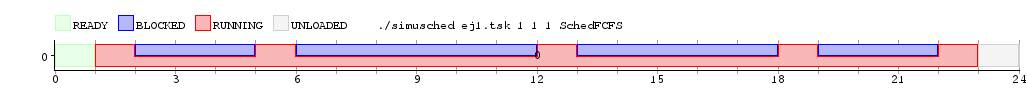
\includegraphics[width=1\textwidth]{ej1}
            \caption{}
        \end{figure} \\
No son muchas las cosas a revisar, entre ellas: \\
- Las llamadas bloqueantes son, en efecto, 4 \\
- Las llamadas bloqueantes en ning\'un caso duran menos de 2 tiempos \\
- Las llamadas bloqueantes en ning\'un caso se exceden de 7 tiempos de duraci\'on

\end{homeworkProblem}

\clearpage
\begin{homeworkProblem}[Ejercicio 2]
    En este segundo ejercicio estamos a cargo de Rolando, su complejo algoritmo, y sus distracciones al momento de sentarse a la computadora. \\
    Nuestro primer encargo es escribir un lote de tareas que simule la situaci\'on de Rolando descripta en el enunciado. Este lote incluye entonces una primer corrida de 100 ciclos de CPU en ning\'un caso bloqueantes buscando simular los 100 ciclos de corrida del algoritmo complejo de Rolando. Nos valemos para ello de la funci\'on provista \textit{TaskCPU}. Lo siguiente ser\'an 2 tareas con llamadas bloqueantes de una duraci\'on variable dentro de un rango; en otras palabras, 2 tareas que realizan exactamente aquello que se nos pidi\'o en el primer ejecicio del trabajo pr\'actico. Usamos entonces la tarea \textit{TaskConsola} con los par\'ametros correspondientes para simular las tareas de ocio de Rolando. \\
    
    \textbf{Gr\'aficos utilizando 1 y 2 n\'ucleos} \\
    Los gr\'aficos a continuaci\'on (\textit{Figura 2}) corresponden a la ejecuci\'on de la simulaci\'on utilizando el algoritmo \textbf{FCFS} para 1 core (Figura 2) y para 2 cores (Figura 3). En ambos casos el costo de cambio de contexto es de 4 ciclos.
    
    \begin{figure}[h]
        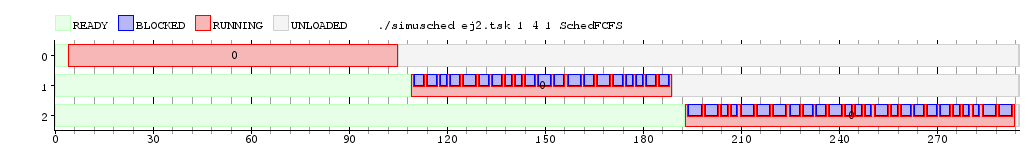
\includegraphics[width=1\textwidth]{ej2-1core}
        \caption{}
    \end{figure}
    
    \begin{figure}[h]
        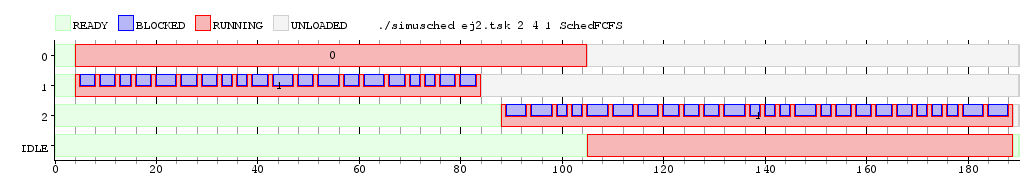
\includegraphics[width=1\textwidth]{ej2-2core}
        \caption{}
    \end{figure}

    \textbf{Latencia} \\
    La siguiente asignatura es el c\'alculo de la latencia de cada una de las tareas en cada uno de los dos casos anteriores:
\begin{table}[h]
  \begin{center}
\begin{tabular}{c|c|c|c}
        & Tarea 0 & Tarea 1 & Tarea 2 \\
\hline
1 core  & 4       & 109     & 193     \\
\hline
2 cores & 4       & 4       & 88     
\end{tabular}
  \end{center}
\end{table}

\textbf{Desventajas} \\
Hablar de desventajas suena a poco: si lo Rolando cuenta con una computadora de un n\'ucleo que usa un algoritmo de scheduling \textbf{FCFS}, va a tener que matar su aburrimiento con alguna otra actividad que no incluya la computadora en la que est\'a corriendo su complejo algoritmo, ya que ning\'un otro proceso va a tener CPU disponible para comenzar a ejecutar. En otras palabras, Rolando no podr\'a reproducir ning\'un tema musical hasta que el algoritmo no concluya. Esta circunstancia se puede llegar a apreciar en el gr\'afico correspondiente a la ejecuci\'on de la simulaci\'on utilizando el algoritmo \textbf{FCFS} para 1 core (Figura 2), en donde el primer proceso (proceso 0) se ejecuta de corrido, sin parar ni dejar posibilidad de ejecuci\'on a otros procesos. La diferencia es m\'as notable considerando e gr\'afico correspondiente a la ejecuci\'on de la simulaci\'on utilizando el algoritmo \textbf{FCFS} para 2 cores (Figura 3) en donde la existencia de un core extra implica la posibilidad de que (a lo sumo) un proceso distinto del proceso 0 pueda ser ejecutado sin necesidad de esperar la conclusi\'on del primero.
    
    
\end{homeworkProblem}

\clearpage
\begin{homeworkProblem}[Ejercicio 3]
    El tercer ejercicio nos invita a programar \textbf{TaskBatch}, esto es, una tarea que realiza \textit{cant\_bloqueos} llamadas bloqueantes en momentos elegidos de forma pseudoaleatoria, y que utilice \textit{total\_cpu} ciclos de reloj. \\
    
    \textbf{Implementaci\'on} \\
Para la implentaci\'on de la tarea pedida utilizamos 2 vectores: \\
- el primero de ellos es un vector de booleanos (de nombre \textit{ticks} en el c\'odigo) y nos permiti\'o discretizar el tiempo que la tarea debe permanecer corriendo. Tiene tama\~no \textit{total\_cpu}, y cada posici\'on representa un ciclo de reloj. ticks[i] es \textbf{true} si y s\'olo si durante el ciclo \textit{i} la tarea se bloquea \\
- mientras que el segundo, \textit{posTiempo}, es un vector de enteros de mismo tama\~no que \textit{ticks} inicializado con el valor correspondiente a la posici\'on en cada caso. \\ 
Es posible que se trate de detalles poco significativos de la implementaci\'on, pero si llegamos hasta ac\'a, los mencionamos: lo que hacemos es desordenar \textit{posTiempo} y asignar el valor \textbf{true} a cada una de las posiciones de \textit{ticks} correspondientes a los primeros \textit{cant\_bloqueos} valores de \textit{posTiempo}. \\
Como hicimos anteriormente, las llamadas bloqueantes las implementamos usando la funci\'on \textit{uso\_IO}, mientras que aquellas no bloqueantes usando \textit{uso\_CPU}. \\

    \textbf{Gr\'afico} \\
A continuanci\'on (Figura 4) exponemos el gr\'afico resultado de de un lote de 3 tareas \textbf{TaskBatch} con diferentes par\'ametros (distinta duraci\'on y distinta cantidad de bloqueos en cada caso) y \textbf{FCFS} como scheduler. \\
        \begin{figure}[h]
            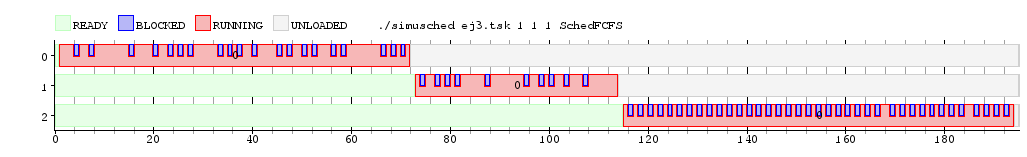
\includegraphics[width=1\textwidth]{ej3}
            \caption{}
        \end{figure} \\
No se nos sugiri\'o ninguna catidad de cores en particular, de modo que elegimos 1 core como opci\'on para nuestra corrida. Esto se puede apreciar notando la ejecuci\'on secuencial de las tareas, que en ning\'un caso arrancan sin que la tarea que las precede concluya. 


\end{homeworkProblem}

\clearpage
\begin{homeworkProblem}[Ejercicio 4]
    El cuarto ejercicio no solicita m\'as que la implementaci\'on del scheduler \textit{Round-Robin} siguiendo algunas aclaraciones. EOM
\end{homeworkProblem}

\clearpage
\begin{homeworkProblem}[Ejercicio 5]
    La consigna del quinto ejercicio de este trabajo empieza de la siguiente forma:
    \begin{displayquote}
Dise\~ne un lote con 3 tareas de tipo \textbf{TaskCPU} de 50 ciclos y 2 de tipo \textbf{TaskConsola} con 5 llamadas blooqueantes de 3 ciclos de duraci\'on cada una. Ejecutar y graficar la simulaci\'on utilizando el scheduler \textit{Round-Robin} con quantum 2, 10 y 50.
    \end{displayquote}
Figura 5 corresponde al gr\'afico de la simulaci\'on hecha utilizando un quantum de 2. Figura 6 y Figura 7 corresponden a los gr\'aficos de las simulaciones hechas con 10 y 50 quantums respectivamente. \\
        \begin{figure}[h]
            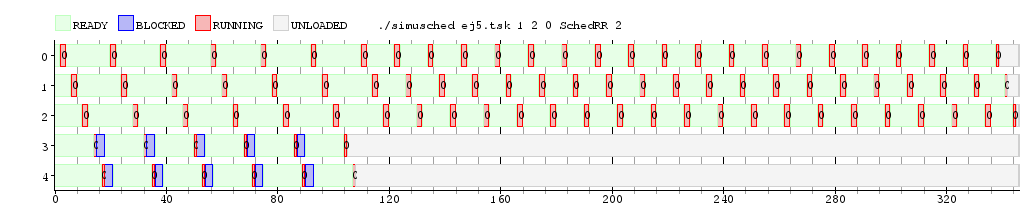
\includegraphics[width=1\textwidth]{ej5-2q-1c}
            \caption{}
        \end{figure} \\
        \begin{figure}[h]
            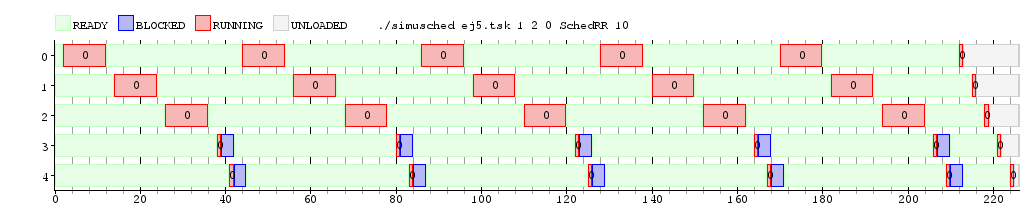
\includegraphics[width=1\textwidth]{ej5-10q-1c}
            \caption{}
        \end{figure} \\
        \begin{figure}[h]
            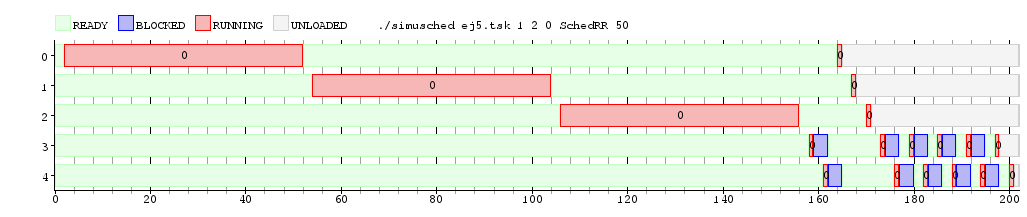
\includegraphics[width=1\textwidth]{ej5-50q-1c}
            \caption{}
        \end{figure} \\
    
    \textbf{Latencia, waiting time y tiempo total de ejecuci\'on} \\
    Sigamos adelante con la segunda parte del ejercicio.
        \begin{displayquote}
Con un cambio de contexto de 2 ciclos y un s\'olo n\'ucleo calcular la \textit{latencia}, el \textit{waiting time} y el tiempo total de ejecuci\'on de las cinco tareas para cada quantum.
    \end{displayquote}


\begin{table}[h]
\centering
\begin{tabular}{c|c|c|c|c|c|c|c}
           & Tarea 0 & Tarea 1 & Tarea 2 & Tarea 3 & Tarea 4 & Total   & Promedio \\
\hline           
Quantum 2  & 2       & 6       & 10      & 14      & 17      & 49      & 9,8      \\
\hline
Quantum 10 & 2       & 14      & 26      & 38      & 41      & 121     & 24,2      \\
\hline
Quantum 50 & 2       & 54      & 106     & 158     & 161     & 481     & 96,2    
\end{tabular}
\caption{Latencia}
\end{table}
\begin{table}[h]
\centering
\begin{tabular}{c|c|c|c|c|c|c|c}
           & Tarea 0 & Tarea 1 & Tarea 2 & Tarea 3 & Tarea 4 & Total   & Promedio \\
\hline
Quantum 2  & 289     & 292     & 295     & 84      & 87      & 1047      & 209,4      \\
\hline
Quantum 10 & 162     & 165     & 168     & 201     & 204      & 900      & 180      \\
\hline
Quantum 50 & 114     & 117     & 120     & 177     & 180      & 708      & 141      \\
\end{tabular}
\caption{Waiting time}
\end{table}
\begin{table}[h]
\centering
\begin{tabular}{c|c|c|c|c|c|c|c}
           & Tarea 0 & Tarea 1 & Tarea 2 & Tarea 3 & Tarea 4 & Total   & Promedio \\
\hline
Quantum 2  & 339     & 342     & 345     & 105     & 108      & 1239      & 247,8      \\
\hline
Quantum 10 & 213     & 216     & 219     & 222     & 225      & 1095      & 219      \\
\hline
Quantum 50 & 165     & 168     & 170     & 198     & 201      & 902      & 180,4      \\
\end{tabular}
\caption{Tiempo total de ejecuci\'on}
\end{table}


Finalmente:
\begin{displayquote}
\mbox{¿}En cu\'al es mejor cada uno? \mbox{¿}Por qu\'e ocurre esto?
    \end{displayquote}
Afinemos el l\'apiz a partir de los n\'umeros en las tres tablas anteriores y tratemos de entender qu\'e ocurre en cada caso. Empezamos por la latencia, que parece el m\'as evidente. Como podemos ver (Cuadro 1), la relaci\'on es lineal: a menor quantum, menor latencia. Parece razonable este comportamiento, basta pensar en qu\'e entendemos cuando hablamos de \textit{quantum}: un menor quantum es en definitiva un menor tiempo de CPU para cada proceso en cada una de las \textit{iteraciones}. Pero esto no es otra cosa que, dado un proceso cualquiera, (con un costo de cambio de contexto fijo para hacer las comparaciones, como es el caso) menor tiempo de espera hasta ser \textit{atendido} por primer vez, ya que todos los procesos que lo precedean en el orden de obtenci\'on de recursos de ejecuci\'on \textit{tardan} menos. En otra forma de exponerlo, consideremos un proceso cualquiera $$p_{i}$$Sea i su \textit{turno}, es decir, el orden asignado por el scheduler para ser atendido. Hay \textit{i} - 1 procesos que tendr\'an CPU antes que aquel que consideramos. Luego, su latencia estar\'a dada por la suma de \textit{i} - 1 cambios de contexto (esto es un n\'umero fijo, seg\'un mencionamos) m\'as a lo sumo \textit{i} - 1 veces el quantum definido. Es por ello que disminuir el quantum disminuir\'a el segundo sumando, resultando en una menor latencia. \\
Los an\'alisis respecto del waiting time y el tiempo total de ejecuci\'on son similares, ya que (aunque bien podr\'iamos no saberlo de forma anticipada) el tiempo de ejecuci\'on que necesitan los procesos definidos es siempre el mismo. Al cambiar el quantum que se asigna, lo que hacemos es modificar la forma (temporal) de atender esas necesidades de procesamiento, no as\'i el tiempo de procesamiento que le llevar\'a a los procesos concluir su tarea. Lo que puede concluirse viendo los resultados (Cuadro 2 y Cuadro 3) es que a mayor quantum, menor waiting time y tiempo total de ejecuci\'on. Una vez m\'as, este resultado es razonable. Considerando fuertemente la aclaraci\'on respecto de la nula variaci\'on del tiempo efectivo de procesamiento, lo que var\'ia entonces es el tiempo que un proceso espera estando listo. Este tiempo de espera es una suma de 2 valores: por un lado, el \textit{tiempo efectivo de espera}, es decir, el tiempo que efectivamente un proceso espera que otro proceso libere CPU, y costo de los cambios de contexto, por otro. Como el \textit{tiempo efectivo de espera} es inevitable, dada la limitante en los recursos de procesamiento, lo \'unico que puede reducirse es el costo de los cambios de contexto. \mbox{¿}C\'omo reducimos el costo de los cambios de contexto? Cambiando de contexto lo menos posible. \mbox{¿}C\'omo cambiamos de contexto lo menos posible? Asignando un quantum mayor, seg\'un se verifica en los resultados.



\end{homeworkProblem}

\clearpage
\begin{homeworkProblem}[Ejercicio 6]
    Work in progress...
\end{homeworkProblem}

\clearpage
\begin{homeworkProblem}[Ejercicio 7]
    Work in progress...
\end{homeworkProblem}

\clearpage
\begin{homeworkProblem}[Ejercicio 8]
    En este punto, se nos asignó la tarea de implementación de un scheduler Round-Robin que no permita la migración de procesos
entre núcleos. La asignación de CPU se realizaría en el momento de carga de un proceso y el núcleo correspondiente al mismo sería aquel con menor cantidad de procesos activos totales.

\bigskip

\textbf{Implementación}

La implementación de este scheduler no difiere mucho del de la del ejercicio 4, sólo que en este caso se tiene una cola de procesos por CPU. Además, se posee un entero por CPU (en un vector) que indica la cantidad de procesos activos para cada uno de estos, a ser utilizados cuando se cargue un proceso nuevo. Por último, poseemos un mapa de procesos para saber a qué CPU corresponde cada uno.

Al cargar un proceso, se obtiene el índice (CPU) del mínimo elemento del vector de "activos" y con eso se empuja el proceso a la cola correspondiente y se aumenta la cantidad de activos. Por último, se agrega el proceso con su CPU al mapa de procesos.

Al hacer un tick, la única diferencia con el código del ejercicio 4, además de elegir la cola correspondiente al cpu indicado, es al momento de finalización de una tarea. En este caso, se le resta uno a la cantidad de activos del CPU y se elimina al proceso del mapa de procesos. Luego, es análogo.

Al desbloquearse un proceso, simplemente se obtiene el CPU del mismo a través del mapa de procesos. Con esto, se empuja al proceso al core correspondiente.

\bigskip

\textbf{Ejemplo 1}

Un escenario en el que este scheduler es peor en contraposición con el Round-Robin tradicional, es cuando se van alternando procesos de corta duración con procesos que tarden bastante, como por ejemplo sería el caso de INSERTE EJEMPLO DE LA VIDA REAL AQUÍ. En este caso, terminarían primero los procesos de corta duración, quedando CPUs sin ningún proceso asignado; no se estarían utilizando, realentizando el tiempo de compleción de los procesos y probablemente su tiempo de espera. Sin embargo, la latencia no se vería afectada y sería la misma en ambos casos.

Para ejemplificar esto, construimos un lote de 7 tareas "TaskCPU", alternadas en tiempos de 1 y 8 ciclos. A continuación, se presenta un gráfico de tal lote que simula la situación planteada:

\begin{figure}[h]
    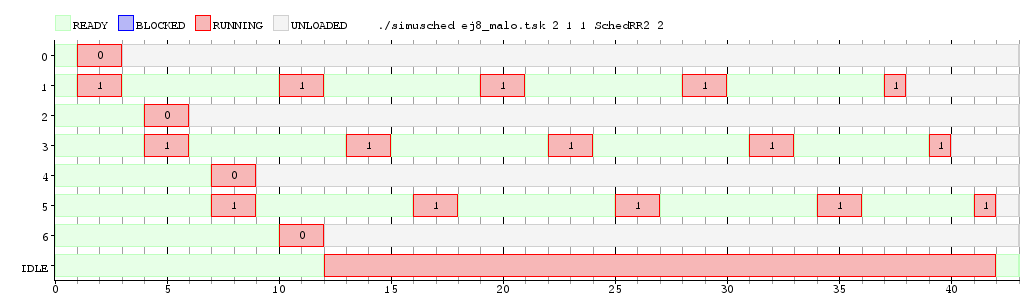
\includegraphics[width=1\textwidth]{ej8MaloRR2}
    \caption{Ejecución en Round-Robin 2}
    \label{RR2Malo}
\end{figure}

Como se muestra en la figura \ref{RR2Malo}, podemos notar lo antes mencionado. Con este nuevo scheduler, a partir del instante 16, el CPU 0, ya no posee ninguna tarea a ejecutar, siendo que terminaron todas las que fueron asignadas al mismo al momento de carga. Por lo tanto, queda en IDLE, mientras que el CPU 1 ejecuta alternadamente los 3 procesos restantes.

En la siguiente tabla mostramos distintas métricas, correspondientes a esta simulación:
% Tabla RR2
\begin{table}[h]
  \caption{Ejecución en Round-Robin 2}
  \centering
    \begin{tabular}{c c c c c}
    \hline
          & Latencia & Espera & Compleción & Ratio (E/C) \\
    \hline
        0 &     1    &    1   &      3     &     0.333   \\
        1 &     1    &   29   &     38     &     0,763   \\
        2 &     4    &    4   &      6     &     0.666   \\
        3 &     4    &   31   &     40     &     0.775   \\
        4 &     7    &    7   &      9     &     0.777   \\
        5 &     7    &   33   &     42     &     0,785   \\
        6 &     10   &   10   &     12     &     0.833   \\
        AVG & 4,857  & 16,428 &   21,428   &     0,705   \\
    \end{tabular}
\end{table}


En cambio, en la figura \ref{RRMalo} (que se presenta a continuación), podemos observar, como con el Round-Robin tradicional, cuando terminan de ejecutarse las tareas cortas (0, 2, 4 y 6), el CPU 1 sigue siendo utilizado por las restantes. Notar que aunque perdemos 1 ciclo extra por cada cambio de CPU, los procesos siguen terminando antes que con el nuevo scheduler implementado.

\begin{figure}[h]
    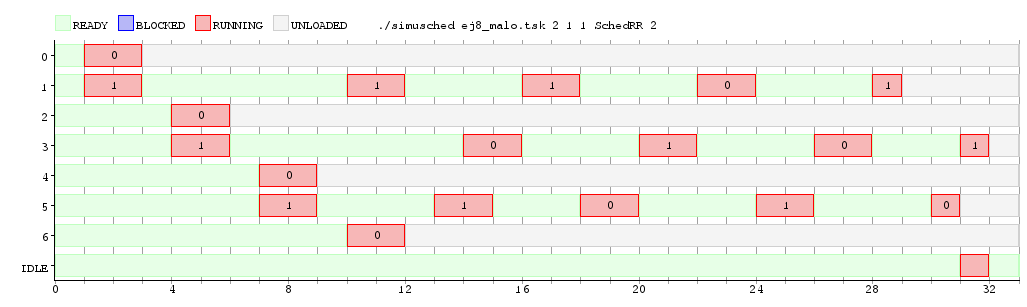
\includegraphics[width=1\textwidth]{ej8MaloRR}
    \caption{Ejecución en Round-Robin Tradicional}
    \label{RRMalo}
\end{figure}

En la siguiente tabla volcamos datos con las mismas métricas que en la tabla correspondiente a \textit{Round-Robin 2}.

% Tabla RR1
\begin{table}[h]
  %\captionsetup{justification=justified,singlelinecheck=false}
  \caption{Ejecución en Round-Robin Tradicional}
  \centering
    \begin{tabular}{c c c c c}
    \hline
          & Latencia & Espera & Compleción & Ratio (E/C) \\
    \hline
        0 &     1    &    1   &      3     &    0.333    \\
        1 &     1    &   20   &     29     &    0,690    \\
        2 &     4    &    4   &      6     &    0.666    \\
        3 &     4    &   23   &     32     &    0,719    \\
        4 &     7    &    7   &      9     &    0.777    \\
        5 &     7    &   22   &     31     &    0,710    \\
        6 &     10   &   10   &     12     &    0.833    \\
        AVG & 4,857  & 12,429 &   17,428   &    0,675    \\
    \end{tabular}
\end{table}

Como supusimos anteriormente, podemos ver como el tiempo de espera y compleción de los procesos largos es menor en \textit{Round-Robin Tradicional}, por lo que en promedio también es mejor. La latencia se mantiene estable.

\bigskip

\textbf{Ejemplo 2}

Sin embargo, este nuevo tipo de scheduler resulta útil en algunas situaciones. Tal es el caso cuando se quisiera lanzar un proceso que ejecute en tiempo real. A modo ilustrativo, en el ejemplo anterior, podría el usuario querer ejecutar alguna especie de simulación de física. Imaginemos que ya se terminaron de ejecutar los procesos cortos y queda un core libre. Entonces, la simulación correría sin interrupciones, y aunque llegaran más procesos, en principio caerían probablemente  en el mismo CPU (si los otros procesos no terminaron), pero estaría balanceado. El tiempo de espera sería menor, como probablemente también la latencia de la simulación.

Para reflejar este comportamiento, modificamos el lote de tareas anterior, agregando la tarea 7 (TaskCPU de 12 ciclos) en el momento 4. Además, agregamos dos tareas pequeñas más que interrumpen a la tarea 7. El gráfico correspondiente se encuentra a continuación:

\begin{figure}[h]
    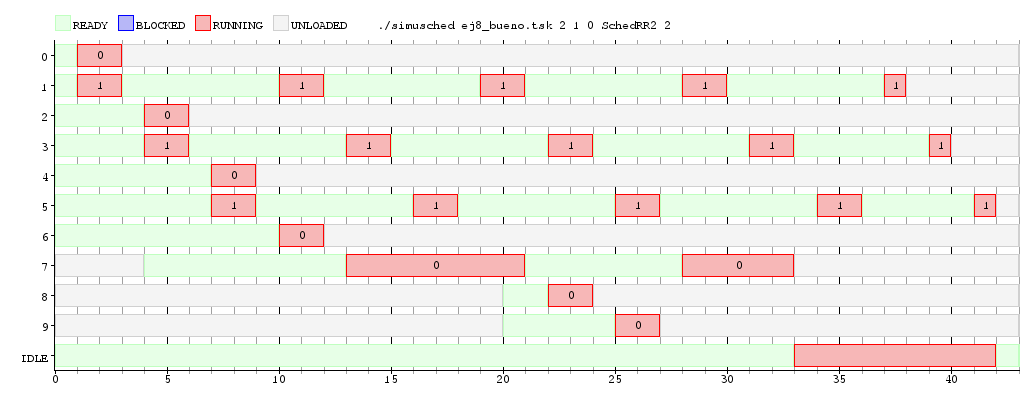
\includegraphics[width=1\textwidth]{ej8BuenoRR2}
    \caption{Ejecución en Round-Robin 2}
    \label{RR2Bueno}
\end{figure}

Como mencionamos, si bien la tarea 7 es interrumpida, tiene un corto tiempo de espera (7 ciclos). Compararlo con la figura \ref{RR2Malo} que se presenta a continuación:

\begin{figure}[h]
    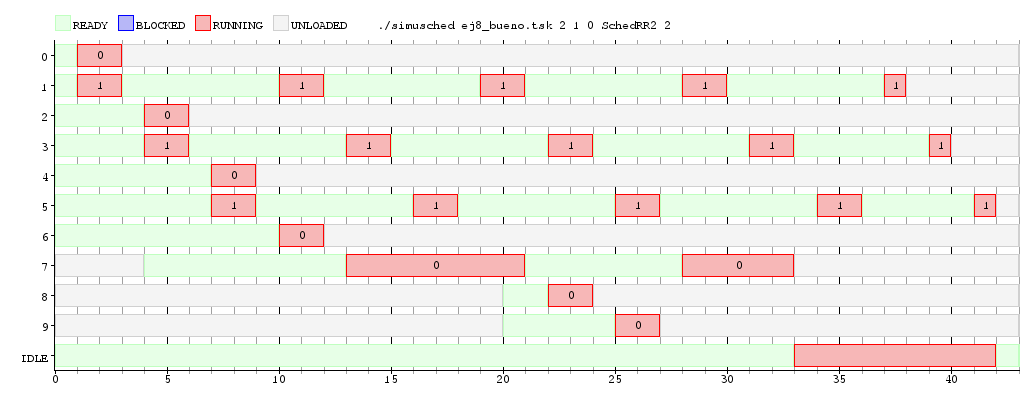
\includegraphics[width=1\textwidth]{ej8BuenoRR2}
    \caption{Ejecución en Round-Robin Tradicional}
    \label{RR2Malo}
\end{figure}

Si bien la tarea 7 tiene la misma latencia en ambos casos, el tiempo de espera es mucho mayor en el \textit{Round-Robin Tradicional}. Como sólo nos importa esta tarea realmente, presentamos una tabla comparativa entre ambos Schedulers para la tarea 7.

\begin{table}[h]
  \caption{Comparación entre schedulers para la tarea 7}
  \centering
    \begin{tabular}{c c c c c}
    \hline
            & Latencia & Espera & Compleción & Ratio (E/C) \\
    \hline
        RR  &     1    &   15   &     28     &    0.536    \\
        RR2 &     1    &    7   &     20     &    0.35     \\
    \end{tabular}
\end{table}

Notar que si no existieran las tareas 8 y 9 que interrumpen ó si hubiera un core libre, la espera sería 0. Igualmente, es notable la mejora que provee el nuevo scheduler en esta situación particular.

Además de esto, en la realidad hay otros factores a considerar que no podrían ser medidos con la simulación utilizada. Por ejemplo, en arquitecturas SMP, es importante mantener cierta afinidad al procesador asignado al proceso, para aprovechar la caché. Si hubiera cambio de procesador, el proceso llegaría con la caché vacía, produciéndose un miss y teniendo que ir a buscar los datos a memoria principal. A esto se le suma el tiempo de los cambios de procesador y de contexto que no son despreciables. En ese sentido, el nuevo scheduler sería preferible al \textit{Round-Robin Tradicional}.

\end{homeworkProblem}


\end{spacing}
\end{document}

%%%%%%%%%%%%%%%%%%%%%%%%%%%%%%%%%%%%%%%%%%%%%%%%%%%%%%%%%%%%%

%----------------------------------------------------------------------%
% The following is copyright and licensing information for
% redistribution of this LaTeX source code; it also includes a liability
% statement. If this source code is not being redistributed to others,
% it may be omitted. It has no effect on the function of the above code.
%----------------------------------------------------------------------%
% Copyright (c) 2007, 2008, 2009, 2010, 2011 by Theodore P. Pavlic
%
% Unless otherwise expressly stated, this work is licensed under the
% Creative Commons Attribution-Noncommercial 3.0 United States License. To
% view a copy of this license, visit
% http://creativecommons.org/licenses/by-nc/3.0/us/ or send a letter to
% Creative Commons, 171 Second Street, Suite 300, San Francisco,
% California, 94105, USA.
%
% THE SOFTWARE IS PROVIDED "AS IS", WITHOUT WARRANTY OF ANY KIND, EXPRESS
% OR IMPLIED, INCLUDING BUT NOT LIMITED TO THE WARRANTIES OF
% MERCHANTABILITY, FITNESS FOR A PARTICULAR PURPOSE AND NONINFRINGEMENT.
% IN NO EVENT SHALL THE AUTHORS OR COPYRIGHT HOLDERS BE LIABLE FOR ANY
% CLAIM, DAMAGES OR OTHER LIABILITY, WHETHER IN AN ACTION OF CONTRACT,
% TORT OR OTHERWISE, ARISING FROM, OUT OF OR IN CONNECTION WITH THE
% SOFTWARE OR THE USE OR OTHER DEALINGS IN THE SOFTWARE.
%----------------------------------------------------------------------%
